\documentclass[10pt]{article}
\usepackage[english]{babel}
\usepackage[utf8]{inputenc}
\usepackage{amsmath}
\usepackage{amsfonts}
\usepackage{graphicx}
\usepackage[colorinlistoftodos]{todonotes}
\usepackage{cite}

\title{Progress report: \\
	Repair probabilities for the RCL polymer with two DSBs}
\author{Ignacio Madrid}

\begin{document}

\maketitle

\tableofcontents

\clearpage

\section{Motivation}
Double Strand Breaks (DSB) are a highly cytotoxic type of DNA damage that occur when both strands of duplex DNA break, for instance, after ionizing radiation and cancer chemotherapy. Two principal pathways of DSB repair have evolved: non-homologous end joining (NHEJ) and homologous recombination (HR). NHEJ is the major pathway of DSB repair and consists on the synapsis and ligation of the broken ends. Here, we aim to simulate and study the repair and misrepair rates after two DSBs, via the NHEJ pathway. Polymer models (and in particular, a generalization of the Gaussian chain, the Randomly Cross-Linked (RCL) Polymer) will be used as a model of the chromatin. Stochastic simulations of molecular dynamics will be performed with the goal of characterize the factors that contribute to interfere or improve the repair probability, namely: the distance between the DSBs, the degree of folding of the polymer (simulated by the number of cross-links connecting non-neighbor monomers) and the dispersion effect induced by the DNA repair machinery (simulated by exclusion forces and the local removal of cross-links in the damage foci).

\section{Methods}
 
 \subsection{The RCL polymer}
 To simulate the chromatin we consider the model of a randomly cross-linked (RCL) polymer. An RCL polymer is formed by a chain of $N$ monomers connected by harmonic springs of constant $\kappa$ as backbone, and $N_c$ extra cross-links (CLs) which connect non-neighbor monomers with springs of constant $\kappa'$. CLs are added uniformly over all $\frac{(N-1)(N-2)}{2}$ combinations of non-neighbor monomer pairs. We also define the RCL polymer connectivity $\xi$ as the fraction of added cross-links with respect to the total number of possible pairings, i.e. $\xi = \frac{2N_c}{(N-1)(N-2)}$. 
 
 We characterize the RCL polymer by two $N \times N$ admittance (Laplacian) matrices: the Rouse matrix $M$ which describes the backbone, and $B$ which describes the added connectors. A Laplacian matrix results from the difference between the diagonal degree matrix $D$ that accounts for the total number of connections each monomer has, and the adjacency matrix $A$ that accounts for the connectivity ($A_{m,n} = 1$ if monomers $m$ and $n$ are connected, $0$ otherwise). So
 \begin{equation}
 M_{m,n} = (D_{\text{backbone}} - A_{\text{backbone}})_{m,n} = \begin{cases}
 -1 & \text{ if } |m-n| = 1 \\
 - \sum_{i=1, i \neq n}^{N} M_{i,n}  & \text{ if }m=n \\
 0  & \text{ otherwise }
 \end{cases}
 \label{eqn:Mmatrix}
 \end{equation}
 and, analogically
  \begin{equation}
  B_{m,n} = (D_{\text{CLs}} - A_{\text{CLs}})_{m,n} = \begin{cases}
  -1 & \text{ if $m$ and $n\neq m$ are connected by a CL} \\
  - \sum_{i=1, i \neq n}^{N} B_{i,n}  & \text{ if }m=n \\
  0  & \text{ otherwise }
  \end{cases}
  \label{eqn:Bmatrix}
  \end{equation}

%  So $B$ is constructed stochastically as
%    \begin{equation}
%    B_{m,n} =  \begin{cases}
%    -1 & \text{ with probability $\xi$ , if $|m-n|>1$} \\
%    0 & \text{ with probability $1 - \xi$ , if $|m-n|>1$} \\
%    - \sum_{i=1}^{N} B_{i,n}  & \text{ if }m=n \\
%    0  & \text{ otherwise }
%    \end{cases}
%    \label{eqn:Bmatrix_construction}
%    \end{equation}

An schematic illustration of an RCL polymer is described in Fig. \ref{fig:model}-A along with its respective Laplacian matrices (Fig.\ref{fig:model}-B). 
 
 \subsection{Langevin dynamics of the RCL polymer}
  We supposed the RCL polymer subdued to Langevin dynamics, i.e., if monomer positions of the polymer in time $t$ are represented by the $N \times 3$ matrix $(R_t)_{t\geq0} = (R_1, ..., R_N)_{t\geq0}$ with each $R_i \in \mathbb{R}^3, i = 1,...,N$, the dynamics are described by Eq. \eqref{eqn:general_langevin}:
 
 \begin{equation}
 dR_t = -\frac{1}{\zeta} \nabla \phi(R_t) dt + \sqrt{2D} dW_t
 \label{eqn:general_langevin}
 \end{equation}
 
 where $\zeta$ is the friction coefficient, $\phi$ is an harmonic potential, $D$ is the diffusion coefficient and $(W_t)_{t \geq 0}$ is a $N \times 3$-dimensional Brownian motion. 
 
 The harmonic potential of a RCL polymer is given by the classical Rouse potential and by the potential induced by the random cross-links:
 
 \begin{align}
 \phi(R) &= \frac{\kappa}{2} \sum_{n = 1}^{N-1} ||R_{n+1} - R_{n}||^2 + \frac{\kappa'}{2} \sum_{i,j \in \mathcal{R}} ||R_{i} - R_{j}||^2 \nonumber \\
 &=\frac{\kappa}{2} \text{tr}(R^TMR) + \frac{\kappa'}{2} \text{tr}(R^TBR) 
 \label{eqn:potential}
 \end{align}

 where $\kappa$ and $\kappa' $ are spring constants we will suppose equal,  $\mathcal{R}$ is the set of monomers which have been randomly connected, and $M$ and $B$ are the Laplacian matrices introduced in Eq. \ref{eqn:Mmatrix} and Eq. \ref{eqn:Bmatrix}. Since $\frac{\kappa}{\gamma} = \frac{3D}{b^2}$ where $b$ is the standard deviation of the bonds length, we'll consider the matrix equation:
 
 \begin{equation}
 dR_t = -\frac{3D}{b^2} (M + B) R_t dt + \sqrt{2D} dW_t
 \label{eqn:langevin}
 \end{equation}
 
In the following, we implement the Euler's scheme of Eq. \ref{eqn:langevin}, setting $D = 0.008 \ \mu^2$m/s and $b = 0.2 \ \mu$m. When it is important, the $\Delta t$ used in the discretization of Eq. \ref{eqn:langevin} will be specified. $\Delta t = 0.005 $ sec will be the usual value. Anyhow, to assure numerical stability, condition in Eq. \ref{eqn:stabilityCondition} must always be verified [Ref].

\begin{equation}
\sqrt{2D\Delta t} \leq c \Delta r ^\star
\label{eqn:stabilityCondition}
\end{equation}

 In Eq. \ref{eqn:stabilityCondition}, $\Delta r^\star$ stands for the smallest spatial scale used (it will normally be the monomers encounter distance as it is defined later on) and $c$ is a confidence factor that will be set at $c = 0.2$ in the simulations.
 
  \subsection{Useful statistical properties of the RCL polymer}
  Some useful statistical properties will be measured to study the polymer repair. For instance, the Mean Radius of Gyration (MRG) will be computed as a proper indicator of the polymer compaction. The MRG is defined as the root mean square distance from each monomer to the center of mass of the polymer (Eq. \ref{eqn:mrg}).
  
  \begin{equation}
  \text{MRG}(R) = \sqrt{\frac{1}{N} \sum_{m=1}^{N}(R_m - \bar{R})^2}
  \label{eqn:mrg}
  \end{equation}
  
  It has been proven \cite{pre2017} that for a given connectivity fraction $\xi$ and when the connectivity is low ($N_c \ll \frac12 N^2$) the mean square radius of gyration MSRG (MRG$^2$) can be approximated by Eq. \ref{eqn:msrg_xi}.
  
   \begin{equation}
   \text{MSRG}(\xi) \approx \frac{3b^2}{4(1-\xi)\sqrt{N \xi}}
   \label{eqn:msrg_xi}
   \end{equation}
  
  
 \subsection{Induction of Double Strand Breaks (DSBs)}
 In particular, we are interested on the probability of repair after two DSBs. One DSB (damage focus \guillemotleft A\guillemotright) will be randomly induced between neighbor monomers $A_1$ and $A_2 = A_1 + 1$, where $A_1 \sim \mathcal{U}[1,N-g-2]$. The other DSB (damage focus \guillemotleft B\guillemotright) will be induced in neighbor monomers $B_1$ and $B_2$. A deterministic inter-break genomic distance $g$ will be imposed between A and B, defined as the shortest distance between the DSBs along the backbone, i.e. $g = B_1 - A_2$. An scheme of two DSBs is represented in Fig. \ref{fig:model}-C.  The two breaks define thus three interconnected fragments: the upstream fragment (formed by monomers $1$ to $A_1$), the central fragment (monomers $A_2$ to $B_1$) and the downstream fragment (monomers $B_2$ to $N$).
 
\subsection{Definition of encounter times and probabilities}
 We define the first encounter time between monomers $m$ and $n$ as
\begin{equation}
T_{m,n}^{\epsilon} := \inf \{ t \geq 0 : ||(R_m)_t - (R_n)_t|| < \epsilon  \}
\label{eqn:encountertime}
\end{equation}
where $\epsilon$ is the encounter distance. Then, the repair probability is defined as
$$
\mathbb{P}(\text{Repair}) = \mathbb{P}(\inf \{ T_{A_1,A_2}^\epsilon,  T_{B_1,B_2}^\epsilon \} \leq \inf \{ T_{A_1,B_1}^\epsilon , T_{A_1,B_2}^\epsilon , T_{A_2,B_1}^\epsilon , T_{A_2,B_2}^\epsilon \} )
$$
and the First Encounter Time (FET) as:
$$
\text{FET} = \inf \{ T_{A_1,A_2}^\epsilon,  T_{B_1,B_2}^\epsilon, T_{A_1,B_1}^\epsilon , T_{A_1,B_2}^\epsilon , T_{A_2,B_1}^\epsilon , T_{A_2,B_2}^\epsilon \}
$$

We remark that when monomers are well mixed, the expected repair probability is $2/6 = 1/3$ (favorable encounters / total possible encounters).

\subsection{Simulation of chromatin decondensation around DSBs: Removal of CLs and Excluded Volume Interactions}
It has been reported that the DNA repair machinery induces a relaxation of the chromatin around damage foci (DF) [Ref]. To simulate this dispersion two effects are considered independently: the removal of CLs in the damage foci to induce decompactation of the polymer around the breaks; and the addition of an exclusion potential around the damaged monomers, to simulate self-avoidance towards the cut ends. 

In general, excluded volume forces are added to the polymer dynamics through a new harmonic potential $\phi_{ev}$ that is added to the potential $\phi$ defined in Eq. \ref{eqn:potential}:

\begin{equation}
\phi_{ev}(R) = - \frac{\kappa_{ev}}{2} \sum_{i,j \ : \ i \neq j} ||R_i - R_j ||^2 1_{||R_i - R_j || < \sigma}
\end{equation}
where $\sigma$ is a cutoff radius of exclusion and $1_{||R_i - R_j || < \sigma} = 1$ if $||R_i - R_j || < \sigma$ and $0$ otherwise.

In our case, to simulate the dispersion of chromatin around DSBs only, we induce volume exclusion for the DF monomers only and take $\kappa_{ev} = \kappa$:

\begin{equation}
\phi_{local-ev}(R) = - \frac{\kappa_{ev}}{2} \sum_{i \in \text{DF}}\sum_{j \neq i} ||R_i - R_j ||^2 1_{||R_i - R_j || < \sigma}
\end{equation}

\begin{figure}[!h]
\centering
\includegraphics[width=\textwidth]{../drawings/model4.png}
\caption{Model of an RCL polymer for chromatin repair simulations. \textbf{A}: Example of the Rouse backbone with some cross-links. \textbf{B}: Laplacian matrices of the RCL polymer represented in \textbf{A}: the Rouse matrix ($M$) and the CLs matrix ($B$). \textbf{C}: Scheme of the induction of two DSBs $A$ and $B$ at a distance $g$. \textbf{D}: To simulate the effect of the sparsity induced by the repair machinery, excluded volume forces are added in the damage foci and the concerned CLs are removed.}
\label{fig:model}
\end{figure}

Finally, considering that in spite of the exclusion induced by repair proteins, the whole repair machinery looks for affine ends to join them, we'll consider repair exclusion spheres that repel all monomers except the other cut ends. So, if any two cut ends approach they won't feel exclusion forces. This new exclusion potential is defined in Eq. \ref{eqn:repair_sphere}.

\begin{equation}
\phi_{\substack{repair \\ sphere}}(R) = - \frac{\kappa_{ev}}{2} \sum_{i \in \text{DF}}\sum_{j \notin \text{DF}} ||R_i - R_j ||^2 1_{||R_i - R_j || < \sigma}
\label{eqn:repair_sphere}
\end{equation}

Thereby, volume exclusion potentials originate a new Laplacian $E$ as defined in Eq. \ref{eqn:Ematrix}, that will be added to the Laplacian matrices considered up to now (Eq. \ref{eqn:langevin}):

\begin{equation}
  E_{m,n} = \begin{cases}
  -1 & \text{ if } m \in \text{DF , } n \notin \text{DF  and  }||R_m - R_n || < \sigma  \\
  -1 & \text{ if } n \in \text{DF , } m \notin \text{DF  and  }||R_m - R_n || < \sigma  \\
  - \sum_{i=1,\ i\neq n}^{N} E_{m,i}  & \text{ if }m=n \\
  0  & \text{ otherwise }
  \end{cases}
  \label{eqn:Ematrix}
\end{equation}

So when exclusion forces are considered the simulated system will subdue the dynamic described by Eq. \ref{eqn:langevin_VE}.

 \begin{equation}
 dR_t = -\frac{3D}{b^2} (M + B + E) R_t dt + \sqrt{2D} dW_t
 \label{eqn:langevin_VE}
 \end{equation}

We call the total $M+B+E$ the total Laplacian matrix of the system. The two decondensation effects are summarized in Fig. \ref{fig:model}-D.

\subsection{Scaling distances under condensation: $\xi$-adaptive encounter distances and exclusion radii}

As indicates Eq. \ref{eqn:msrg_xi} (cf. Fig. \ref{fig:mrg_v_nc} for an empirical example), as $N_c$ (equivalently $\xi$) increases the polymer compaction increases too. Since the spatial scale of a compact polymer is different from the spatial scale used by a decompacted polymer, and thus for the same $\varepsilon$, an encounter which is rare enough for the later might be too common for the former, for a more compact polymer, smaller spatial scales should be used. In effect, scaling $\varepsilon$ and $\sigma$ for different degrees of compaction will allow to measure the repair rates conditionally to the compaction, invariantly to the polymer size. So $\varepsilon$ and $\sigma$ will be redefined to be $\xi$-adaptive and preserve the spatial scale. 
Thus, $\varepsilon$ and $\sigma$ will be proportional to the polymer mean size, and in particular, to the MRG. Starting from Eq. \ref{eqn:msrg_xi} we will define the adaptive encounter distance $\tilde{\varepsilon}(\xi)$ as in Eq. \ref{eqn:adaptive_eps}, and the adaptive cutoff radius of exclusion $\tilde{\sigma}(\xi)$ as in Eq. \ref{eqn:adaptive_sigma}, where $v>1$ is a factor which indicates how much bigger is the exclusion sphere with respect to the encounter distance.

\begin{eqnarray}
\tilde{\varepsilon}(\xi) &=& 2 \sqrt{  \frac{3b^2}{N(1-\xi)\sqrt{y^2-1}} }
\label{eqn:adaptive_eps} \\
y &=& 1 + \frac{N \xi}{2(1-\xi)} \nonumber
\end{eqnarray}

\begin{equation}
\tilde{\sigma}(\xi) = v \cdot \tilde{\varepsilon}(\xi)
\label{eqn:adaptive_sigma}
\end{equation}

\subsection{Pipeline of the simulations}
A number $I$ of independent polymer realizations will be simulated to extract mean statistical properties and the repair probabilities conditional to the parameters defined so far. The main pipeline of each realization goes as described below:

\begin{enumerate}
	\item \textbf{Initialization of the polymer backbone} from a random walk in $\mathbb{R}^3$ where each step is i.i.d. $\mathcal{N}(0,b^2)$.
	\item \textbf{Predefinition of DSBs $A$ and $B$}. We take $A_1 \sim \mathcal{U}[1,N-g-2]$ and then $A_2 = A_1 + 1$, $B_1 = A_2 + g$, $B_2 = B_2 + 1$.
	\item \textbf{Induction of random cross-links}. $N_c$ cross-links are induced between non-neighbor monomers such that after breaks $A$ and $B$ the polymer rests fully connected. In practice, we make random connections until obtaining one which verifies the full connectivity condition.
	\item \textbf{Relaxation}. Once the polymer is validly cross-linked, the polymer is subdued to Langevin dynamics (discretized as an Euler's scheme for Eq. \ref{eqn:langevin}) until relaxation time $\tau$, which is computed analytically [Ref] as:
	$$
	\tau = \frac{...}{...}
	$$
	\item \textbf{DSBs Induction and actualization of the total Laplacian matrix}. When the polymer reaches relaxation time, the two cuts are induced between the predefined monomers $A_1$, $A_2$ and $B_1$, $B_2$. Removed bonds are thus cleaned out from the Laplacian matrix. Besides, if CLs are removed from the separated monomers and if Volume Exclusion is included, those effects are also added to the Laplacian as in Eq. \ref{eqn:langevin_VE}.
	\item \textbf{Waiting}. As a way to exclude the repair events which happen immediately after the break, and since the DNA repair is not instantaneous (it requires the arrival of specific proteins to the cut ends), the polymer is let to evolve under Eq. \ref{eqn:langevin} for some waiting time $T_{wait}$
	\item \textbf{Simulation until encounter}. Once $T_{wait}$ is reached, simulation continues until an encounter, as defined in Eq. \ref{eqn:encountertime}, happens between any of the cut ends. If two or more pairs of monomers encounter at the same simulated instant, we randomly choose over those pairs to be the first encounter. If no encounters occur before a threshold time $T_{max}$ the simulation is discarded.
	\item Statistical properties and the encounter event that occurred (repair or misrepair) are saved and a new polymer is initialized to perform the same simulation. 
\end{enumerate}
Finally, the conditional probability of repair is estimated as
$$
\mathbb{P}(\text{Repair}|\Theta) = \frac{\text{Number of $A_1$-$A_2$ or $B_1$-$B_2$ encounters}}{\text{Total number of encounters}}
$$
where $\Theta$ summarizes the experiment parameters, $$\Theta = (N,b,N_c,g,\varepsilon,\sigma,T_{wait},T_{max}).$$

\clearpage

\section{Results}

\subsection{First Encounter Time (FET) distribution when CLs are kept and removed in the damage foci}

Since the FET distribution can be approximated by a single exponential \cite{amitai12}, an exponential function with parameters $a, \lambda$ such that $t \mapsto a \exp(- \lambda t)$ is fitted to the frequency histograms, aiming to compare the $\lambda$ fitted in each one of the experiments sets.

\begin{figure}[h!]
	\centering
	\includegraphics[width=\textwidth]{../DNA_Religation/figures/FEThistograms_keepingANDremoving.png}
	\caption{Distribution of the first encounter time keeping and removing the cross-links in the cleaved monomers. An exponential function has been fitted to each histogram. $N = 100$ monomers, $N_c = 5$, $g = 10$,  $T_{wait} = 25 sec$, and $T_{max} = 60 sec$.}
	\label{fig:hists}
\end{figure}

The results in Fig. \ref{fig:hists} indicate that the removal of cross-links does not seem to affect the mean first encounter time, the estimated rate parameter ($\lambda$) is 0.08 for both cases. Nonetheless, it's no surprising considering that for $N = 100$ and $N_c = 5$ the mean number of connectors in the DF is about $0.4$, so the removal of CLs is not actually occurring for the majority of cases. To overcome this situation and to properly study the effect of removing the CLs a new Laplacian matrix will be included, which will impose a certain number $N_{d}$ of extra cross-links in the DF monomers. Fig. \ref{fig:hists_CLinDF} shows the difference in the FET distributions when we impose $N_d = 2$ CLs in the DF. We can see that when we remove the 2 imposed CLs the mean FET increases in 2 seconds, and the repair rate increases as well. We also observe that when we remove the CLs the most common misrepair corresponds to the looping of the central segment of the broken polymer ($A_2$-$B_1$). In the spirit way Fig. \ref{fig:meanFET_vs_Nd} shows that increasing the imposed $N_d$ reduces the mean FET when those CLs are kept, but not when they are removed. 

In the following, we will determine the effect of the removal of CLs with respect to the inter-break distance $g$ and the number of random CLs $N_c$.

\begin{figure}[h!]
	\centering
	\includegraphics[width=\textwidth]{../DNA_Religation/figures/eventsandFET_005epsilon_CLinDF.PNG}
	\caption{Distribution of the first encounter times and events, keeping and removing the cross-links when imposing CLs in the DF. Both results corresponds to $I = 500$ simulations, with $N = 100$, $N_c = 12$, $N_d = 2$, $g = 10$, $\varepsilon = 0.05 \mu$m, $T_{max} = 45$ sec, $T_{wait} = 2.5$ sec and $\sigma = 0$ (no volume exclusion). \textbf{A}: Schematic representation of the experimental set and possible encounters. \textbf{B}: Results keeping CLs in DF. \textbf{1.} Histogram of relative frequencies and fitted exponential function, with and estimated rate of 0.096 and a mean FET of $12.600 \pm 1.032$ sec. \textbf{2.} Encounter events distribution. \textbf{C}: Results removing CLs in DF. \textbf{1.} Histogram of relative frequencies and fitted exponential function, with and estimated rate of 0.077 and a mean FET of $14.171 \pm 1.117$ sec. \textbf{2.} Encounter events distribution.}
	\label{fig:hists_CLinDF}
\end{figure}

\begin{figure}[h!]
	\centering
	\includegraphics[width=\textwidth]{../DNA_Religation/projects/RCLPolymer_CLs@DamageFoci/figures/mFET_keepingVSremovingCL.PNG}
	\caption{Mean FET as function of $N_d$ when CLs in the DF are kept and removed. $N_c = 12$ and $\varepsilon$ is $(N_c+N_d)$-adaptive, ranging from 0.096 $\mu$m ($N_d = 0$) to 0.088 $\mu$m ($N_d = 5$).}
	\label{fig:meanFET_vs_Nd}
\end{figure}


%It should be noted that since the maximum time of simulation is set at 60 seconds (i.e. if nothing happens in 60 seconds the simulation is discarded) the distribution is biased and corresponds to $\mathcal{L}(FET|FET<60)$. For instance, when the simulation maximum time has been increased to 200 seconds, the rate parameter is estimated at 0.04.


%Finally as we see in figure \ref{fig:hists2} within the misrepair events, the mismatchs seems to be equidistributed. 

%\begin{figure}[h!]
%	\centering
%	\includegraphics[width=\textwidth]{../DNA_Religation/figures/eventsRepartition.png}
%	\caption{Distribution of the first encounter time keeping the CLs in the damage foci, and distribution of the repair and misrepair events (1000 realisations).}
%	\label{fig:hists2}
%\end{figure}

\clearpage

\subsection{Changes on the repair probability conditionally to $g$, $N_c$ and decondensation}

\subsubsection{Effect of $g$ on the repair probability}

\begin{figure}[h]
	\centering
	\includegraphics[width=\textwidth]{../DNA_Religation/projects/RCLPolymer_Repair_Probability/Figures/proba_v_g__100monomers_keepingandremovingCLs_xxlarge.png}
	\caption{Repair probability as function of the genomic distance $g$ between the two DSBs. $N = 100$, $N_c = 15$, $\varepsilon = 0.1 \mu$m and $N_d = 0$ (no CLs imposed in DF).}
	\label{fig:proba_v_g_1}
\end{figure}

Fig. \ref{fig:proba_v_g_1} shows that regardless the removal of cross-links, repair probability increases as the inter-break genomic distance increases. 
%So, removing the cross-links in the disconnected monomers does not seem to induce a better repair probability


Besides, when we keep CLs in the DF, we can remark an important gap between the probabilities at $g = 1$ (i.e., the two DSBs are connected, $A2$ and $B1$ being neighbors) and the other genomic distances (Fig. \ref{fig:proba_v_g_1} Zoom). As only valid cuts are allowed (the polymer rests fully connected after the breaks) the central segment is indeed connected to the upstream and/or the downstream fragment. The probability of being connected to only one of them is higher than the probability of being connected to both, so the segment could be pushed towards one of the free monomers rapidly and then induce a good ratio of repair. This case will be treated as an out-layer from now on, and thus the following comparative analysis will be performed for $g\geq 2$.

Fig. \ref{fig:proba_v_g_1} does not show any significant difference for the removal of CLs, because no CLs were imposed in the DF. However, imposing $N_d = 2$, as in Fig. \ref{fig:proba_v_g_Nd2} and \ref{fig:all_v_g}, shows that the removal of DSB' CLs helps the reparation for distant breaks. Nonetheless, near breaks ($g < 10$) seems to perform better reparation rates when the CLs are kept in the DF. Fig. \ref{fig:all_v_g} complements Fig. \ref{fig:proba_v_g_Nd2} and show the effect of $g$ and the removal of CLs in other observables (the MSRG at encounter time, the mean FET and the fitted rate parameter $\lambda$ to the FET distribution). We observe that at encounter time the MSRG is, as expected, bigger when we remove CLs (the polymer is more decompacted). We also see that removing CLs extend the FET. 

\begin{figure}[h!]
	\centering
	\includegraphics[width=\textwidth]{../DNA_Religation/figures/proba_v_g_Nd2_zoom.png}
	\caption{Repair probability as function of $g$  when $N = 100$, $N_c = 15$, $\varepsilon = 0.1 \mu$m and $N_d = 2$ (2 CLs imposed in DF) which are kept (blue) or removed (orange) after the induction of the DSBs. ($I = 500$ simulations)}
	\label{fig:proba_v_g_Nd2}
\end{figure}


\begin{figure}[h!]
	\centering
	\includegraphics[width=\textwidth]{../DNA_Religation/figures/__v_g_keepANDremove.png}
	\caption{Repair probability (A), MSRG at encounter time (B), mean FET (C) and estimated encounter rate parameter ($\lambda$) (D) as functions of $g$  when $N = 100$, $N_c = 15$, $\varepsilon = 0.1 \mu$m and $N_d = 2$ (2 CLs imposed in DF). A window zooming in $g \in [2,11]$ with 500 simulations for each $g$ is at the right of each graph.} 
	\label{fig:all_v_g}
\end{figure}



\subsubsection{Effect of $N_c$ on the repair probability}

Increasing the number of cross-links approaches the simulated probabilities to $1/3$, which is the result expected in the well mixed case, as we observe in Fig. \ref{fig:proba_v_cl}. Indeed, increasing the number of CLs and therefore approaching all monomers not only increases the chances of repair, but also of mismatch. It is interesting that systems which had a repair probability $\leq 1/3$  because had DSBs at a very small genomic distance ($g \leq 3$) (so the chances of a bad matching were higher) improve their repair probabilities when we increase the number of cross-links. 

In effect, increasing the number of random connectors increases as well the compactness of the polymer, revealed as a decrease of the mean radius of gyration (Fig. \ref{fig:mrg_v_nc}). Besides, we can see that the position of the breaks does not affect the ensemble mean of the gyration radius. 

In conclusion, \textbf{the compactness help to repair polymers cut in a small neighborhood.} This is coherent with which was observed in Fig. \ref{fig:all_v_g}-A, where at small genomic distances, the repair probabilities were better when CLs were kept in the DF. On the other hand, at a big genomic distance ($g = 20$), it can be observed in Fig. \ref{fig:proba_v_NcNd} that the presence of CLs in the DBS' monomers swifts the repair probabilities down, although the removal of those CLs after the break.

\begin{figure}[h!]
	\centering
	\includegraphics[width=\textwidth]{../DNA_Religation/projects/RCLPolymer_Repair_Probability/Figures/proba_v_Nc__100monomers_01eps_removingCLs_500iteration_goodDT.png}
	\caption{Repair probability as a function of $N_c$ for $N=100$, $\varepsilon = 0.1 \mu$m and $N_d$ = 0. If any, CLs are removed in DF.}
	\label{fig:proba_v_cl}
\end{figure}

\begin{figure}[h!]
	\centering
	\includegraphics[width=\textwidth]{../DNA_Religation/projects/RCLPolymer_Repair_Probability/Figures/MRG_vs_CLnumber_3genomicdistances.png}
	\caption{Polymer of 100 monomers. Mean radius of gyration in function of the number of cross-links.}
	\label{fig:mrg_v_nc}
\end{figure}



\begin{figure}[h!]
	\centering
	\includegraphics[width=\textwidth]{../DNA_Religation/projects/RCLPolymer_CLs@DamageFoci/figures/proba_vs_NcNd.png}
	\caption{Repair probability in function of the total number of polymer CLs ($N_c + N_d$) where $N_d$ is fixed to 0 (blue) and 1 (orange). In both cases, CLs are removed from the DF monomers, $N = 100$, $g = 20$, $\epsilon = \tilde{\varepsilon}(\xi)$ according to Eq. \ref{eqn:adaptive_eps} and the step $\Delta t$ is also adapted such that Eq. \ref{eqn:stabilityCondition} remains verified.}
	\label{fig:proba_v_NcNd}
\end{figure}


\subsubsection{Effect of volume exclusion on the repair probability}

 Larger values of $\sigma$ make the waiting for looping times last longer (Fig. \ref{fig:mFET_v_Nc_EV}) and thus make the encounter events rarer, however they do not affect dramatically the repair probability overall (Fig. \ref{fig:vs_volumeexclusionradius}). 


\begin{figure}[h]
	\centering
	\includegraphics[width=\textwidth]{../DNA_Religation/projects/RCLPolymer_ExcludedVolumeExperiments/figures/meanFET_vs_VE_Nc.png}
	\caption{Mean FET in function of $N_c$, with and without an excluded volume of $\sigma =$ 0.1 $\mu$m. $\varepsilon$ is fixed at 0.04 $\mu$m and so, either $\varepsilon$ and $\sigma$ are adapted to the polymer compaction.}
	\label{fig:mFET_v_Nc_EV}
\end{figure}

\begin{figure}[h]
	\centering
	\includegraphics[width=\textwidth]{../DNA_Religation/projects/RCLPolymer_ExcludedVolumeExperiments/figures/proba_vs_cutoffradius_bigfont.png}
	\caption{Probability and 95\% confidence interval of repair, in function of the cutoff radius of volume exclusion.}
	\label{fig:vs_volumeexclusionradius}
\end{figure}

Fig. \ref{fig:MSRGandFET_byEvent} shows that, as expected, the misrepair scenarios are associated with smaller radius of gyration, and thus with more compact polymers. This could be an indication that decondensation of the polymer chain in the damage loci could lead to better repair probabilities. 

\begin{figure}[h]
	\centering
	\includegraphics[width=\textwidth]{../DNA_Religation/projects/RCLPolymer_Repair_Probability/figures/by_event_type_distributions.png}
	\caption{Distribution of the first encounter times and the mean square radius of gyration in repair and misrepair events considering local excluded volume interactions.}
	\label{fig:MSRGandFET_byEvent}
\end{figure}

We can see in Fig. \ref{fig:pr_v_g_cutoffs} that the repair probability in function of the genomic separation between the breaks behaves similarly that previously (cf. Fig \ref{fig:proba_v_g_1}). 

\begin{figure}[h]
	\centering
	\includegraphics[width=\textwidth]{../DNA_Religation/projects/RCLPolymer_Repair_Probability/figures/proba_v_g_VEcutoffs.png}
	\caption{Probability and 95\% confidence interval of repair, in function of interbreak genomic distance for exclusion cutoffs  $b/2$ and $b$ ($b = 0.1 \mu$m).}
	\label{fig:pr_v_g_cutoffs}
\end{figure}

However the repair probability function considering excluded volume interactions is always below the repair probability in the non-excluded case (Figs. \ref{fig:proba_vs_g_exclusion} and \ref{fig:proba_vs_Nc_exclusion})

\begin{figure}[h]
	\centering
	\includegraphics[width=\textwidth]{../DNA_Religation/projects/RCLPolymer_ExcludedVolumeExperiments/figures/proba_vs_genomicDistance_excludedANDnot_01cutoff.png}
	\caption{Probability of repair in function of the genomic separation between the breaks.}
	\label{fig:proba_vs_g_exclusion}
\end{figure}

\begin{figure}[h]
	\centering
	\includegraphics[width=\textwidth]{../DNA_Religation/projects/RCLPolymer_ExcludedVolumeExperiments/figures/proba_v_Nc.png}
	\caption{Probability of repair in function of the number of random cross-links, for two breaks separated by 4 monomers (g=5).}
	\label{fig:proba_vs_Nc_exclusion}
\end{figure}

\begin{figure}[h]
	\centering
	\includegraphics[width=\textwidth]{../DNA_Religation/projects/RCLPolymer_ExcludedVolumeExperiments/figures/proba_v_g_EV_03_20Nc}
	\caption{Probability of repair in function of the genomic separation between the breaks. Even for small genomic distances and high connectivity (20 random cross-links) the local volume exclusion seems to interfere with the correct repair, rather than helping it.}
	\label{fig:proba_vs_g_03exclusion}
\end{figure}

\begin{figure}[h]
	\centering
	\includegraphics[width=\textwidth]{../DNA_Religation/projects/RCLPolymer_ExcludedVolumeExperiments/figures/proba_v_Nc_EV_03_4g}
	\caption{Probability of repair in function of the total number of cross-links, with an inter-break genomic distance $g = 4$. }
	\label{fig:proba_vs_Nc_03exclusion}
\end{figure}


\clearpage

\subsubsection{Effect of volume exclusion with more restrictive encounter distances}

After tracking the inter-break physical distances (in $\mu$m) as it is presented in figure \ref{fig:distances3breaks}, it seems that the encounter distance of 0.1 $\mu$m is rather permissive. So, smaller encounter radius will be considered now to see if excluded volume could help the correct repairs.

\begin{figure}[h]
	\centering
	\includegraphics[width=\textwidth]{../DNA_Religation/projects/DSB_Clustering/figures/distanceBetween3DSBs}
	\caption{Track of the distances between the ends of three DSBs just before the breaks are induced at relaxation time. The ends of the same break tend to be nearer in comparison to the other distances. }
	\label{fig:distances3breaks}
\end{figure}

Figure \ref{fig:noExclusion_002epsilon} shows the results with and without volume exclusion and with a encounter distance of $\varepsilon = b \cdot 10^{-1} = 0.02 \mu$m.

\begin{figure}[h]
	\centering
	\includegraphics[width=\textwidth]{../DNA_Religation/figures/eventsandFET_002epsilon_VE}
	\caption{Encounter results with and without volume exclusion for a two DSBs at a genomic distance of 4 and considering 20 random cross-links. \textbf{a}. Experiment set. \textbf{a}. Encounter events distribution. The most frequent mismatch corresponds to the looping of the central fragment of the broken polymer. \textbf{c}. First Encounter Time distribution of all the events. \textbf{d}. Same results considering volume exclusion with a cutoff radius of 0.1 $\mu$m.}
	\label{fig:noExclusion_002epsilon}
\end{figure}





\clearpage

\subsection{Repair probability in different domains}

We'll now consider a polymer replied in two connected sub-domains (TADs) (figure \ref{fig:TADSmodel}).

\begin{figure}[!h]
	\centering
	\includegraphics[width=\textwidth]{../drawings/twoTADmodel.png}
	\caption{Model of the RCL polymer replied in two connected subdomains.}
	\label{fig:TADSmodel}
\end{figure}


Figure \ref{fig:proba_v_interTADdistance} shows the repair probabilities of two DSBs located at independent connected sub-domains. We see that the correct repair rate is visible higher. The probabilities are observed for two sub-domains where the genomic distance that separate them is increased. The distance between the two sub-domains does not seem to affect the (already good) probability of correct repair. 

The following figures illustrates the following experiment: two DSBs are induced \textbf{in the same sub-domain} with a genomic distance between the breaks as in the previous section. The repair probability is measured again to see if the presence of a juxtaposed sub-domain without breaks affects the repair in the first sub-domain.


\begin{figure}[h]
	\centering
	\includegraphics[width=0.7\textwidth]{../DNA_Religation/projects/RCLPolymer_TwoDomains/figures/RepairProba_v_interTADdistance.png}
	\caption{One DSB in each subdomain (two subdomains of size 50). Repair probability vs. inter-TAD separation distance.}
	\label{fig:proba_v_interTADdistance}
\end{figure}


\begin{figure}[h]
	\centering
	\includegraphics[width=0.7\textwidth]{proba_v_g_2domains.png}
	\caption{Probability and 95\% confidence interval of repair, in function of the interbreak distance for two DSBs induced in one sub-domain of size 100 on a polymer formed by two sub-domains (100 and 50 monomers). The subdomain had 5 RCLs.}
	\label{fig:2domain}
\end{figure}



\begin{figure}[h]
	\centering
	\includegraphics[width=0.7\textwidth]{../DNA_Religation/projects/RCLPolymer_TwoDomains/figures/proba_v_g_2domains_10randomconnectors}
	\caption{Probability and 95\% confidence interval of repair, in function of the interbreak distance for two DSBs induced in one sub-domain of size 100 on a polymer formed by two sub-domains (100 and 50 monomers). The subdomain had 10 RCLs.}
	\label{fig:2domain_10rcls}
\end{figure}


\clearpage


\begin{figure}[h]
	\centering
	\includegraphics[width=0.7\textwidth]{../DNA_Religation/projects/RCLPolymer_TwoDomains/figures/proba_vs_longrange_first}
	\caption{Probability of repair in function of the number of long-range connectors. Two DSBs were induced at a genomic distance of 5 in the first sub-domain of a polymer conformed by 2 sub-domains of 100 monomers with 10 inner cross-links.}
	\label{fig:proba_v_longrange}
\end{figure}

Figures \ref{fig:proba_v_parasytes} and \ref{fig:proba_v_longrange_sizes} suggest that the presence of a juxtaposed cross-linked polymer chain of any size does not affect the repair performance for two DSBs at a given genomic distance when the number of long-range connectors remains little. Figure \ref{fig:proba_v_longrange_3and45} suggest that a higher number of long-range connectors increases the randomness of the system, making the probabilities go to $1/3$. If the correct repair probability was already about $1/3$ without long-range connections (for example, thanks to a high number of intra-domain cross-links), adding the long-range links does not change the repair rates.

\begin{figure}[h]
	\centering
	\includegraphics[width=\textwidth]{../DNA_Religation/projects/RCLPolymer_TwoDomains/figures/proba_vs_genomicdistance_parasytes}
	\caption{Repair probability of a 100-monomers sub-domain with two DSBs, in function of the genomic inter-break distance between the DSBs. Juxtaposed to the broken sub-domain, there is another sub-domain of size 50, 100 and 200 without breaks. The first sub-domain has 10 inner cross-links and the juxtaposed one has a connectivity of 0.2\%. There are no long-range connectors between the two sub-domains.}
	\label{fig:proba_v_parasytes}
\end{figure}

\begin{figure}[h]
	\centering
	\includegraphics[width=\textwidth]{../DNA_Religation/projects/RCLPolymer_TwoDomains/figures/proba_v_longrangeNum_3AND45}
	\caption{Probability of repair in function of the number of long-range connectors. Two DSBs were induced at a genomic distance of 5 in the first sub-domain of a polymer conformed by 2 sub-domains of 100 monomers with 3 and 45 inner cross-links.}
	\label{fig:proba_v_longrange_3and45}
\end{figure}

\begin{figure}[h]
	\centering
	\includegraphics[width=\textwidth]{../DNA_Religation/projects/RCLPolymer_TwoDomains/figures/proba_v_longrangeNum_differentsizes}
	\caption{Probability of repair for 0,2,4 and 6 long-range connectors, and different sizes for the juxtaposed unbroken sub-domain. Two DSBs were induced at a genomic distance of 30 in the first sub-domain (100 monomers). The juxtaposed sub-domain has a constant connectivity fraction (0.2\%).}
	\label{fig:proba_v_longrange_sizes}
\end{figure}






\clearpage

\subsubsection{TODO}
\begin{itemize}
\item For one DSB in each TAD: Simulate the repair probability vs. intra-TAD connectors number
\item For one DSB in each TAD: Simulate the repair probability vs. long-range connectors number
\item For two DSB in a TAD: Compare repair probabilities with the results obtained in the previous section. Does a second TAD (with no breaks) affect the repair probability of the first one? How?
\item THINK ABOUT STOCHASTICALLY GENERATING THE CROSS-LINKS, USING IN THE CONNECTIVITY $\xi$ AS A PROBABILITY SO, INSTEAD OF FIXING THE NUMBER OF CROSS-LINKS WE FIX $\xi$ AND HAVE $\mathbb{E}(Nc) = \xi N_l$ INSTEAD OF A DETERMINISTIC $Nc = \lfloor \xi N_l \rfloor $. THE RCL POLYMER WILL BE THE AN ERDOS-RENYI GRAPH, THE SUB-DOMAINS POLYMER MATRIX WOULD CORRESPOND TO A WELL KNOWN STOCHASTIC BLOCK MODEL, ETC.
\end{itemize}

\clearpage

\section{Partial conclusions}

\begin{itemize}
	\item At short genomic distances ($g < 4$) the removal of CLs in the DF makes FET shorter (or equivalently the encounter rate $\lambda$ higher) and the repair probabilities worse than when CLs are kept in the breaks. At further $g$, the observed behavior is the opposite and the expected one: the removal of CLs makes FET longer, but the repair rates are increased.
\end{itemize}

\begin{itemize}
	\item When the mismatch rate is high (near DSBs and/or high connectivity) the most common misrepair seems to be the $"a_2-b_1$" one, which corresponds to the looping of the central segment of the cut RCL polymer.
	\item Keeping or removing the cross-links in the separated neighbors does not seem to particularly help the repair, at least without considering volume exclusion. The joint action of CLs removal and volume exclusion in the damage foci should be analyzed more carefully to conclude if this "relaxation" helps or not the repair.
	\item If there are enough cross-links, even for DSBs separated by a large genomic distance the repair probability goes down to $1/3$, i.e. the expected value by pure chance. The best correct repair probabilities occur, as one could expect, at large interbreak genomic distances with few random cross-links. However, if the breaks are close and the repair probability is less than $1/3$, the increment of cross-links improves the correct match rate.
	\item Local excluded volume in the damage foci seems to do not affect or even obstruct the repair, rather than improving its probability. Probability curves with local local exclusion volume are indeed down shifted in comparison with the non-excluded ones.
\end{itemize}

\section{Perspectives}
\begin{itemize}
	\item Non-homologous end-joining repair : The repair probability curves in function of the inter-break genomic distance and the number of cross-links reveal a characteristic behavior (tendency to $1/3$ when the connectivity is high, a sort of logistic growth when the genomic distance between the breaks is increased) that could be verified analytically using the results available for the unbroken RCL polymer\footnote{O. Shukron and D. Holcman. Statistics of randomly cross-linked polymer models to interpret chromatin conformation capture data. \textbf{Phys. Rev. E} 2017 Jul:96, 012503}
	\item For the RCL polymer with subdomains : It has been reported that DSBs cluster. In particular, damaged active genes remain largely unrepaired and clustered to be repaired afterwards via homologous recombination in postreplicative cells\footnote{Aymard F. \textit{et al.} Genome-wide mapping of long-range contacts unveils clustering of DNA double-strand breaks at damaged active genes. \textbf{Nat Struct Mol Biol.} 2017 Apr;24(4):353-361}. It could be interesting to study if DSB clustering is a property inherent to the polymer dynamics, and if it is facilitated by exclude volume interactions and the local removal of cross-links in the damage foci.
\end{itemize}

\clearpage

\begin{thebibliography}{10}
	\bibitem{amitai12} Amitai A, Kupka I, Holcman D. Computation of the mean first-encounter time between the ends of a polymer chain. Phys Rev Lett. 2012 Sep 7;109(10):108302.
	\bibitem{pre2017} Shukron, O. and Holcman D. Statistics of randomly cross-linked polymer models to interpret chromatin conformation capture data. Phys. Rev. E 96, 012503 – Published 27 July 2017.
\end{thebibliography}
\end{document}